\section{Scheduling}

\textbf{Was ist Scheduling?}
\begin{itemize}
	\item Zuordnung von Aufträgen (\textbf{Jobs}) zu Arbeitsträgern, z.B. Maschinen, unter Beachtung von Nebenbedingungen zum Optimieren einer oder mehrerer Zielgrößen
\end{itemize}
\bigskip
\textbf{Scheduling Notation:}
\begin{itemize}
	\item $n$ \textbf{Jobs} müssen auf $m$ \textbf{Maschinen} bearbeitet werden
	\item Job $j$ hat auf Maschine $i$ eine \textbf{Prozesszeit} $p_{ij}$
	\item Job $j$ kann ein \textbf{Gewicht} $w_j$ haben $\rightarrow$ Repräsentiert die Wichtigkeit des Jobs
	\item Job $j$ kann einen \textbf{Liefertermin} $d_j$ haben
	\item Notation eines \textbf{Scheduling-Problems}: $\alpha\mid\beta\mid\gamma$
	\begin{itemize}
		\item $\alpha$: Maschinenumgebung
		\item $\beta$: Auftragscharakteristik und Beschränkungen
		\item $\gamma$: Zielgröße
	\end{itemize}
\end{itemize}
\bigskip
\textbf{Performanz-Kenngrößen:}
\begin{itemize}
	\item \textbf{Fertigstellungszeitpunkt (Completion Time) $\boldsymbol{C_j}$}:
	\begin{itemize}
		 \item Zeitpunkt, zu welchem Job $j$ fertiggestellt ist
		 \item Bei mehreren Maschinen $C_{ij}$ (Fertigstellung von Job $j$ auf Maschine $i$) gilt: $C_j=\max\limits_{i\in I}\{C_{ij}\}$
	\end{itemize}  
	\item \textbf{Unpünktlichkeit (Lateness)} $L_j=C_j-d_j$ beschreibt die Abweichung vom Fertigstellungszeitpunkt zum Liefertermin. Negativ, wenn Produkt zu früh fertig
	\item \textbf{Verspätung (Tardiness)} $T_j=\max\{C_j-d_j,0\}$ wie Lateness, aber erlaubt keine negativen Werte
	\item \textbf{Einheits-Strafe (Unit penalty)}  
	$U_j=
	\begin{cases}
		1\;, & \text{wenn } C_j > d_j\\
		0\;, & \text{sonst}
	\end{cases}$
	\newline
	\newline
	erhebt eine Einheitsstrafe, wenn Fertigstellungszeitpunkt zu spät
\end{itemize}
\bigskip
\textbf{Maschinenumgebung $\boldsymbol{(\alpha)}$:}
\begin{itemize}
	\item \textbf{Einzel Maschine} $\boldsymbol{(1)}$
	\item \textbf{Parallele Maschinen $\boldsymbol{(Pm, Qm, Rm)}$:}
	\begin{itemize}
		\item Mehrere Maschinen, die gleichzeitig Jobs abarbeiten
		\item $Pm$: $m$ identische Maschinen (gleiche Geschwindigkeit)
		\item $Qm$: $m$ Maschinen mit unterschiedl., job-unspezifischen Geschwindigkeiten
		\item $Rm$: $m$ Maschinen mit unterschiedl., job-spezifischen Geschwindigkeiten
	\end{itemize}
	\item \textbf{Flow-Shop $\boldsymbol{(Fm)}$}: $m$ Maschinen in Serie, alle Jobs müssen diese durchlaufen (selbe Maschinen-Reihenfolge)
	\item \textbf{Job-Shop $\boldsymbol{(Jm)}$}: $m$ Maschinen, alle Jobs müssen diese durchlaufen, haben jedoch unterschiedliche Maschinen-Reihenfolge
\end{itemize}
\bigskip
\textbf{Auftragscharakteristik $\boldsymbol{(\beta)}$:}
\begin{itemize}
	\item \textbf{Freigabezeiten (Release dates) $\boldsymbol{(r_j)}$}: Auftrag kann nicht vor diesem Zeitpunkt gestartet werden
	\item \textbf{Unterbrechungen (Preemptions) $\boldsymbol{(prmp)}$}: Bearbeitung eines Auftrags kann unterbrochen und später fortgesetzt werden
	\item \textbf{Permutation $\boldsymbol{(prmu)}$}: Job-Reihenfolge auf der ersten Maschine muss beibehalten werden
	\item \textbf{Rüstzeiten (Setup times) $\boldsymbol{(s_{jk}, s_{jk}^i)}$}:
	\begin{itemize}
		\item Bevor mit Auftrag $k$ begonnen werden kann, ist Maschine $i$ durch Umrüstung blockiert
		\item $s_{jk}$: Rüstzeit ist nur von den aufeinanderfolgenden Jobs $j$ und $k$ abhängig
		\item $s_{jk}^i$: Rüstzeit ist zusätzlich von Maschine $i$ abhängig
	\end{itemize}
\end{itemize}
\bigskip
\textbf{Zielfunktion $\boldsymbol{(\gamma)}$:}
\begin{itemize}
	\item \textbf{Makespan $\boldsymbol{(C_{max})}$}: Entspricht Gesamtproduktionszeit, also der Zeit, wenn der letzte Job fertiggestellt ist: $C_{max}=\max\limits_{j\in J}\{C_j\}$
	\item \textbf{Gesamtfertigstellungszeiten (Total completion time) $\boldsymbol{(\sum C_j)}$:} Summe der Fertigstellungszeiten der Jobs
	\item \textbf{Gewichtete Gesamtfertigstellungszeiten (Total weighted completion time) $\boldsymbol{(\sum w_jC_j)}$:} Summe der gewichteten Fertigstellungszeiten der Jobs
	\item \textbf{Gesamtverspätung (Total tardiness) $\boldsymbol{(\sum T_j)}$:} Summe der Verspätungszeiten
	\item \textbf{Anzahl verspäteter Jobs (Number of tardy Jobs) $\boldsymbol{(\sum U_j)}$:} Summe der Einheitsstrafen
\end{itemize}
\bigskip
\textbf{Gantt-Charts:}
\begin{itemize}
	\item Visualisierungsmöglichkeit von Scheduling-Lösungen
	\item Block für die Bearbeitung von Job $j$ auf Maschine $i$ ist auf Höhe von
	$i$ und Länge des Blocks entspricht Prozesszeit $p_{ij}$
	\item Innerhalb des Blocks steht die Job-Nummer oder Prozesszeit (problemabhängig)
\end{itemize}
\begin{center}
	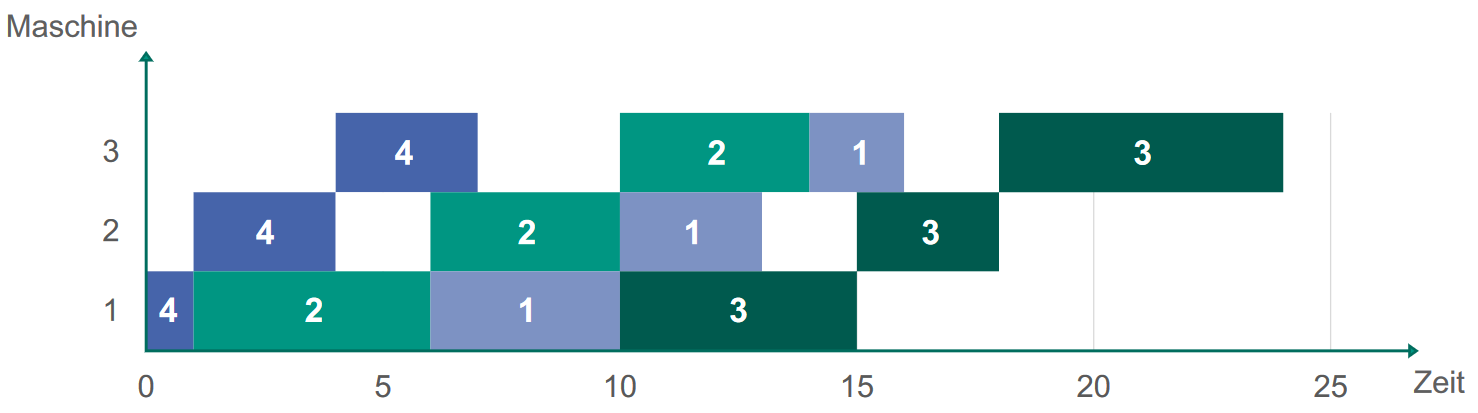
\includegraphics[width=0.7\textwidth]{images/gantt.png}
\end{center}

\subsection{Ein-Maschinen-Probleme}
\begin{itemize}
	\item \textbf{Problemstellung}: $n$ Jobs sollen auf einer Maschine in
	Reihenfolge gebracht werden
	\item Jeder Schedule kann als Permutation der Jobs $1,\ldots,n$ angesehen
	werden \\
	$\rightarrow n!$ verschiedene Schedules
\end{itemize}
\bigskip
\textbf{Minimierung der Fertigstellungszeiten:}
\begin{itemize}
	\item Problem $1\mid\mid C_{max}$ ist trivial, da $C_{max}=\sum\limits_{j=1}^{n} p_j$ für jeden Schedule
	\item Problem $1\mid\mid \sum\limits_{j=1}^{n} C_j$ lässt sich mit \textbf{SPT-Regel} (Shortest Processing Time first) optimal lösen $\rightarrow$ Individuelle Fertigstellungszeitpunkte so gering wie möglich halten
	\begin{center}
		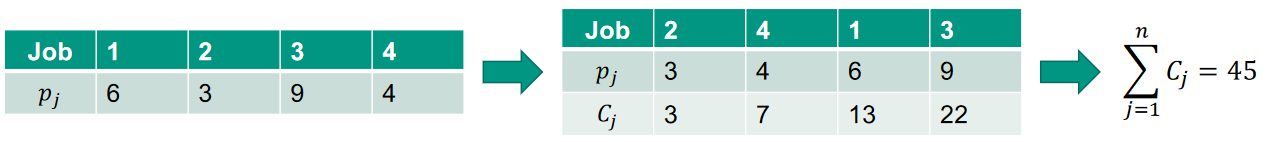
\includegraphics[width=0.8\textwidth]{images/spt.png}
	\end{center}
\end{itemize}
\bigskip
\textbf{Minimierung gewichteter Fertigstellungszeiten:}
\begin{itemize}
	\item Problem $1\mid\mid \sum\limits_{j=1}^{n} w_jC_j$ lässt sich mit \textbf{WSPT-Regel} (Weighted shortest processing time) optimal lösen
	\begin{center}
		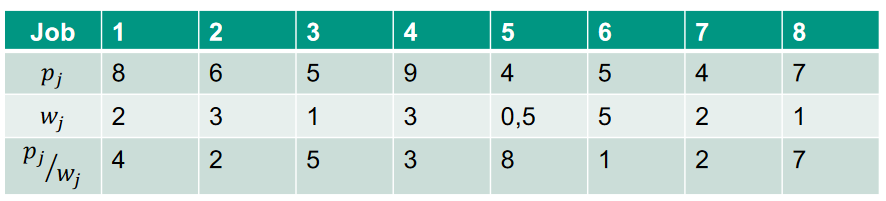
\includegraphics[width=0.7\textwidth]{images/wspt.png}
	\end{center}
	\item Ergebnis: $S=\{6,2,7,4,1,3,8,5\}$ mit $\sum\limits_{j=1}^{n} w_jC_j(S)=329$
\end{itemize}
\bigskip
\textbf{Minimierung der Anzahl verspäteter Jobs:}
\begin{itemize}
	\item Problem $1\mid\mid \sum\limits_{j=1}^{n} U_j$ lässt sich mit \textbf{Moore's Algorithmus} optimal lösen
	\begin{enumerate}
		\item \textbf{Initialisierung}: Sortiere alle Jobs in aufsteigender Reihenfolge nach Lieferterminen $\rightarrow$ Schedule $S$ und setze $J=\emptyset$
		\item \textbf{Job-Auswahl}: 
		\begin{itemize}
			\item Wenn ein verspäteter Job in $S$ existiert $\rightarrow$ Betrachte ersten verspäteten Job $j'$ in $S$ 
			\item Sonst: Gehe zu 4.
		\end{itemize}
		\item \textbf{Job-Entfernung}: Wähle Job $u$ mit größter Prozesszeit, der vor $j'$ kommt und setze $S\coloneqq S\setminus\{u\}$ und $J\coloneqq J\cup \{u\}$
		\item \textbf{Terminierung}: Füge Jobs aus $J$ in beliebiger Reihenfolge an $S$
	\end{enumerate}
	\smallskip
	\begin{center}
		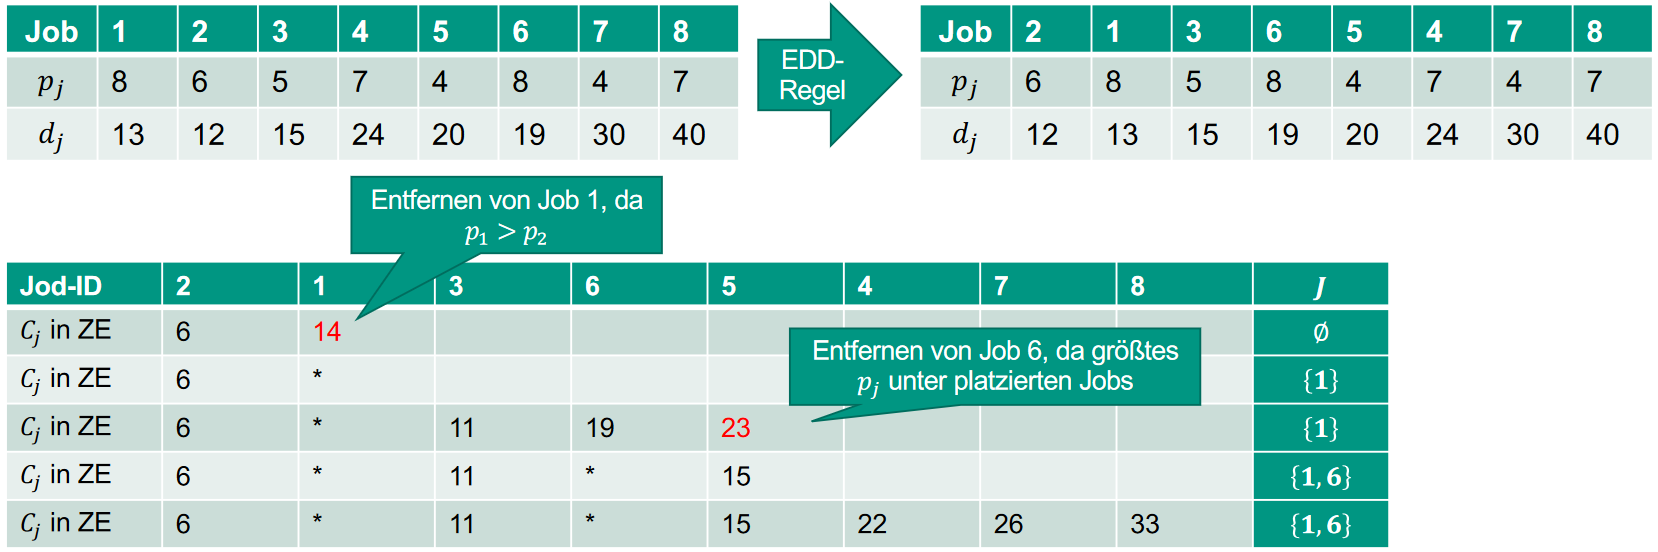
\includegraphics[width=\textwidth]{images/moore.png}
	\end{center}
	\item Ergebnis: $S=\{2,3,5,4,7,8,1,6\}$ oder $S=\{2,3,5,4,7,8,6,1\}$ mit $\sum\limits_{j=1}^{n} U_j(S)=2$
\end{itemize}

\subsection{Flow-Shop-Umgebung}
\begin{itemize}
	\item \textbf{Problemstellung}: $n$ Jobs durchlaufen selbe Maschinensequenz mit $m$ Maschinen. Reihenfolge der Jobabarbeitung kann an jeder Maschine variieren
	\item Unterscheidung nach \textbf{Buffer-Typen}:
	\begin{itemize}
		\item \textbf{Unbegrenzter Zwischenspeicher}: Keine Blockierung vorhergehender Maschinen möglich (\textit{im Folgenden angenommen})
		\item \textbf{Begrenzter Zwischenspeicher}: Blockierung vorhergehender Maschinen möglich, d.h. wenn Produkt auf Maschine 1 fertig ist, dann kann es nicht direkt auf Maschine 2 geschoben werden und blockiert somit Maschine 1
	\end{itemize}
	\item Schedule heißt \textbf{Permutationsschedule}, wenn Jobs in gleicher Reihenfolge auf allen Maschinen abgearbeitet werden
\end{itemize}
\pagebreak
\textbf{Minimierung des Makespan:}
\begin{itemize}
	\item Problem $Fm\mid\mid C_{max}$, wobei $m$ die Anzahl der Maschinen ist
	\item \textbf{Satz}: Für $Fm\mid\mid C_{max}$ existiert für jede Probleminstanz ein optimaler Schedule, bei welchem die Jobsequenz für die ersten zwei Maschinen für die letzten zwei Maschinen gleich ist
	\item \textbf{Folgerung}: Für $F2\mid\mid C_{max}$ und $F3\mid\mid C_{max}$ existieren optimale Schedules die Permutationsschedules sind
	\item Für \textbf{Permutationsschedules} gilt:
	\begin{itemize}
		\item $C_{i,j_1}=\sum\limits_{l=1}^{i}p_{l,j_1}$ für $i=1,\ldots,m$: Fertigstellungszeitpunkt von Job 1 auf Maschine $i$ ist die Summe der Prozesszeiten von Job 1 auf allen vorherigen Maschinen
		\item $C_{1,j_k}=\sum\limits_{l=1}^{k}p_{1,j_l}$ für $k=1,\ldots,n$:
		Fertigstellungszeitpunkt von Job $k$ auf Maschine 1 ist die Summe der Prozesszeiten von allen vorherigen Jobs auf Maschine 1
		\item $C_{i,j_k}=\max\{C_{i-1,j_k},C_{i,j_{k-1}}\}+p_{i,j_k}$ für $i=2,\ldots,m$ und $k=2,\ldots,n$:\\
		Erst, wenn Job $k$ auf vorheriger Maschine $i-1$ fertig ist und wenn Job $k-1$ auf Maschine $i$ fertig ist, kann mit Job $k$ auf Maschine $i$ angefangen werden
	\end{itemize}
	\item $F2\mid\mid C_{max}$ lässt sich mit \textbf{Johnson's Algorithmus} optimal lösen:
	\begin{enumerate}
		\item \textbf{Initialisierung}: Speichere Jobs mit $p_{1,j}\leq p_{2,j}$ in $J_1$ und Jobs mit $p_{1,j}>p_{2,j}$ in $J_2$
		\item \textbf{Job-Sortierung}: Sortiere Jobs in $J_1$ aufsteigend nach Prozesszeiten auf Maschine 1 und Jobs in $J_2$ absteigend nach Prozesszeiten auf Maschine 2
		\item \textbf{Terminierung}: Füge $J_2$ an $J_1$
	\end{enumerate}
	\begin{center}
		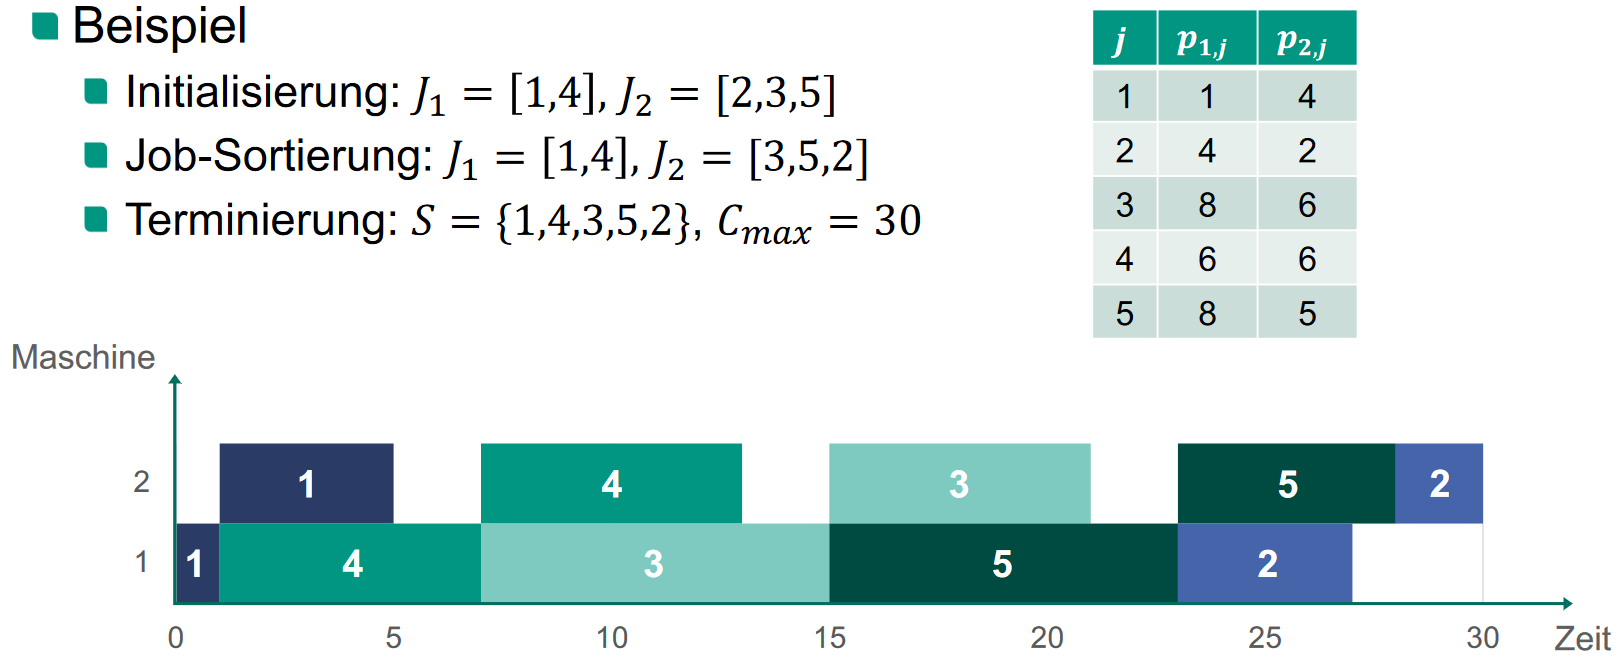
\includegraphics[width=0.75\textwidth]{images/johnson.png}
	\end{center}
\end{itemize}

\textbf{Betrachtung der Komplexität}:
\begin{itemize}
	\item $F2\mid\mid C_{max}$ lässt sich mit Johnson's Algorithmus in \underline{polynomialer Zeit} lösen
	\item $Fm\mid\mid C_{max}$ für $m\geq 3$ ist \underline{NP-schwer} $\rightarrow$ Lösung durch Heuristiken
\end{itemize}
\bigskip
\textbf{Johnson's Algorithmus für 3 Maschinen:}
\begin{itemize}
	\item Für bestimmte Probleminstanzen von $F3\mid\mid C_{max}$ findet eine modifizierte Form von Johnson's Algorithmus ebenfalls eine optimale Lösung
	\item \textbf{Voraussetzung}: $\max\limits_{i\in J}\{p_{2i}\}\leq\min\limits_{k\in J}\{p_{1k}\}$ \underline{oder} $\max\limits_{i\in J}\{p_{2i}\}\leq\min\limits_{k\in J}\{p_{3k}\}$ mit $i\neq k$
	\item \textbf{Vorgehen}: 
	\begin{enumerate}
		\item Berechne $p_{1j}^*=p_{1j}+p_{2j}$ und $p_{2j}^*=p_{2j}+p_{3j}$ für alle $j\in J$
		\item Führe den normalen Johnson Algorithmus für $p_{1j}^*$ und $p_{2j}^*$ durch
	\end{enumerate}
	\begin{center}
		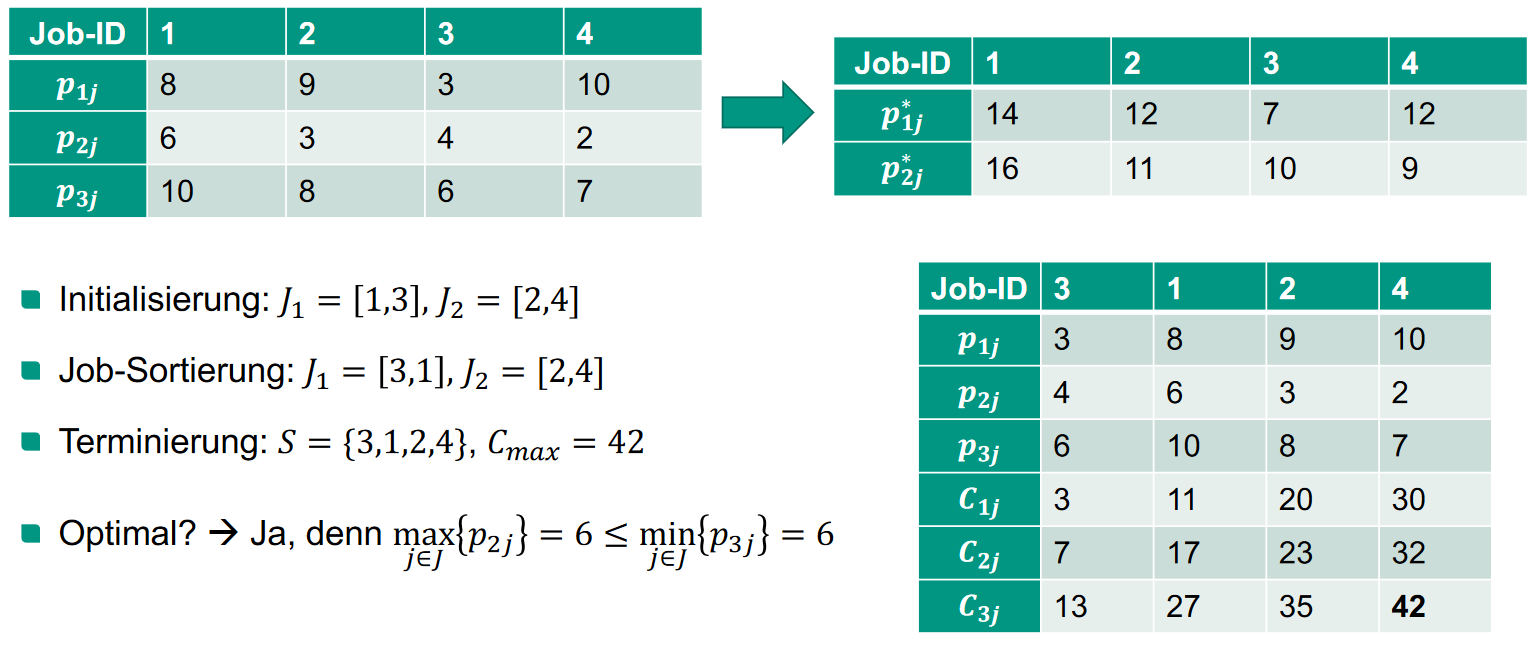
\includegraphics[width=0.8\textwidth]{images/johnson-modified.png}
	\end{center}
	\item Einträge $C_{ij}$ wird nach den Rechenvorschriften für Permutationsschedules (\textit{siehe vorherige Seite}) bestimmt
\end{itemize}
\bigskip
\textbf{Heuristiken:}
\begin{itemize}
	\item Verfahren zur Bestimmung eines zulässigen Punktes eines Problems, dessen Wert möglichst nahe am Optimalwert liegen soll, mit akzeptablem Aufwand
	\item \textbf{Arten von Heuristiken}:
	\begin{itemize}
		\item \textbf{Konstruktionsheuristiken}: Finden eines ersten zulässigen Punktes
		\item \textbf{Verbesserungsheuristiken}: Ausgehend von einem zulässigen Punkt wird nach Verbesserungen gesucht
		\item Heuristiken zur Bestimmung von Schranken
	\end{itemize}
\end{itemize}
\bigskip
\textbf{NEH-Heuristik:}
\begin{enumerate}
	\item Berechne für jeden Job $j$: $T_j=\sum\limits_{i=1}^{m}p_{ij}$
	\item Sortiere Jobs in absteigender Reihenfolge ihrer $T_j$ in einer Liste, wenn mehrere Jobs dieselben Werte für $T_j$ haben, sortiere aufsteigend nach Job-IDs
	\item Nehme die ersten beiden Jobs der Liste und finde die beste Sequenz aus
	diesen Jobs $\rightarrow$ Berechne Makespan für beide möglichen Sequenzen
	und wähle Sequenz mit niedrigerem Makespan. Setze $i\coloneqq 3$
	\item Nehme Job an $i$-te Stelle aus der Liste von Schritt 2. Füge diesen an alle möglichen Positionen der bisher generierten Sequenz ein. Die generierte
	Sequenz, welche den minimalen Makespan aufweist, wird für den nächsten Schritt
	berücksichtigt.
	\item Wenn $i=n \rightarrow \text{Stop}$, sonst $i=i+1$ und gehe zu Schritt 4
\end{enumerate}
\textit{Beispiel siehe Übung, Folie 14-18}
\\

\textbf{MILP für Flow-Shop Maschinenumgebung (allgemein)}:
\begin{itemize}
	\item \textbf{Entscheidungsvariablen}:
	\begin{itemize}
		\item $x_{jk}^{i}$ : Binärvariable: Angabe, ob $j$ vor $k$ auf $i$ produziert wird
		\item $C_{ij}$ : Fertigstellungszeitpunkt von $j$ auf Maschine $i$
	\end{itemize}
	\item \textbf{Zielfunktion}: $Z \rightarrow \min$ mit $Z=\max\limits_{j=1,\ldots,n}\{C_{mj}\}$
	\item \textbf{Nebenbedingungen}:
	\begin{enumerate}
		\item $C_{i j} \geq C_{(i-1) j}+p_{i j}, \forall i=1, \ldots, m ; j=1, \ldots, n$ (Maschinenreihenfolgensicherstellung)
		\item $M \cdot x_{j k}^{i}+C_{i j}-C_{i k} \geq p_{i j}, \forall i=1, \ldots, m ; j=1, \ldots, n-1 ; k=j+1, \ldots, n$ (Jobreihenfolge, wenn $k$ vor $j$)
		\item $M \cdot\left(1-x_{j k}^{i}\right)+C_{i k}-C_{i j} \geq p_{i k}, \forall i=1, \ldots, m ; j=1, \ldots, n-1 ; k=j+1, \ldots, n$ (Jobreihenfolge, wenn $j$ vor $k$)
		\item $Z \geq C_{m j}, \quad \forall j=1, \ldots, n$ (Definition Makespan $Z$)
		\item $C_{0 j}=0, \forall j=1, \ldots, n$ (NNB für virtuelle Maschine $0 \rightarrow$ Job $j$ kann erst ab Zeitpunkt 0 auf Maschine 1 produziert werden)
		\item $x_{j k}^{i} \in\{0 ; 1\}: x_{j k}^{i}=\left\{\begin{array}{l}1, \text { wenn Auftrag } j \text { vor Auftrag } k \text { auf Maschine } i \text{ produziert wird } \\ 0, \text { sonst }\end{array}\right.$
	\end{enumerate}
	\item $M$ ausreichend groß wählen $\rightarrow$ Sorgt für Erfüllung der Ungleichungen, wenn $j$ vor $k$ (2.) oder $k$ vor $j$ (3.) bearbeitet wird
	\item Bei anderer Zielfunktion $\rightarrow$ $Z$ austauschen und 4. eventuell streichen
\end{itemize}
\bigskip
\textbf{MILP für Permutation-Flow-Shop}:
\begin{itemize}
	\item \textbf{Entscheidungsvariablen}:
	\begin{itemize}
		\item $x_{jk}$ : Binärvariable: Angabe, ob $j$ an Position $k$ (auf allen Maschinen) produziert wird
		\item $C_{ik}$ : Fertigstellungszeitpunkt des Jobs auf Position $k$ auf Maschine $i$
	\end{itemize}
	\item \textbf{Zielfunktion}: $Z \rightarrow \min$ mit $Z=\max\limits_{j=1,\ldots,n}\{C_{mj}\}$
	\item \textbf{Nebenbedingungen}:
	\begin{enumerate}
		\item $\sum\limits_{j=1}^{n} x_{j k}=1, \forall k=1, \ldots, n$ (Jede Position hat einen Job)
		\item $\sum\limits_{k=1}^{n} x_{j k}=1, \forall j=1, \ldots, n$ (Jeder Job hat eine Position)
		\item $C_{(i-1) k}+\sum_{j=1}^{n} p_{i j} x_{j k} \leq C_{i k}, \forall i=1, \ldots, m ; k=1, \ldots, n$ (Maschinenreihenfolgensicherstellung)
		\item $C_{i(k-1)}+\sum_{j=1}^{n} p_{i j} x_{j k} \leq C_{i k}, \forall i=1, \ldots, m ; k=1, \ldots, n$ (Jobreihenfolgensicherstellung)
		\item $Z \geq C_{m j}, \quad \forall j=1, \ldots, n$ (Definition Makespan $Z$)
		\item $C_{01}=0$ (NNB für die virtuelle Maschine $0 \rightarrow$ Job auf Position 1 kann erst ab Zeitpunkt 0 auf erster Maschine produziert werden)
		\item $x_{j k} \in\{0 ; 1\}: x_{j k}=\left\{\begin{array}{l}1, \text { wenn Auftrag } j \text { an Position } k \text { produziert wird } \\ 0, \text { sonst }\end{array}\right.$
	\end{enumerate}
	\item Bei anderer Zielfunktion $\rightarrow$ $Z$ austauschen und 5. eventuell streichen
\end{itemize}
\bigskip
\textbf{Flow-Shop-Optimierung durch Solver:}
\begin{itemize}
	\item Obige MILPS können durch Solver (z.B. CPLEX) gelöst werden
	\item Große einfache Probleme $\rightarrow$ Nutze Heuristiken, da diese schneller
	\item Schwere Probleme $\rightarrow$ Nutze Solver
\end{itemize}